\section{Gestión del proyecto}
\label{software}
\noindent En este apartado se expone la planificación seguida en el proyecto, dividido en las tareas que lo componen, mostrando algunas dificultades, problemas y tiempo invertido en cada una de ellas, así como el presupuesto estimado del trabajo realizado.

\subsection{Metodología del software}
\noindent La metodología utilizada en este proyecto ha sido el desarrollo en espiral, en el que cada iteración representa un conjunto de actividades y la siguiente se elige en función del análisis de riesgo de las anteriores. De esta forma, este modelo itera repetidamente mejorando cualquier tipo de conflictos en la implementación, reduciéndolos conforme se completan las iteraciones \cite{boehm1988spiral}.

\subsection{Planificación}

\noindent Para organizar la planificación seguida en este proyecto, se muestra el diagrama de Gantt (figura \ref{fig:gantt}) desde el 07/03/2018 hasta el 06/06/2018: \\

\begin{figure}[H]
	\centering
	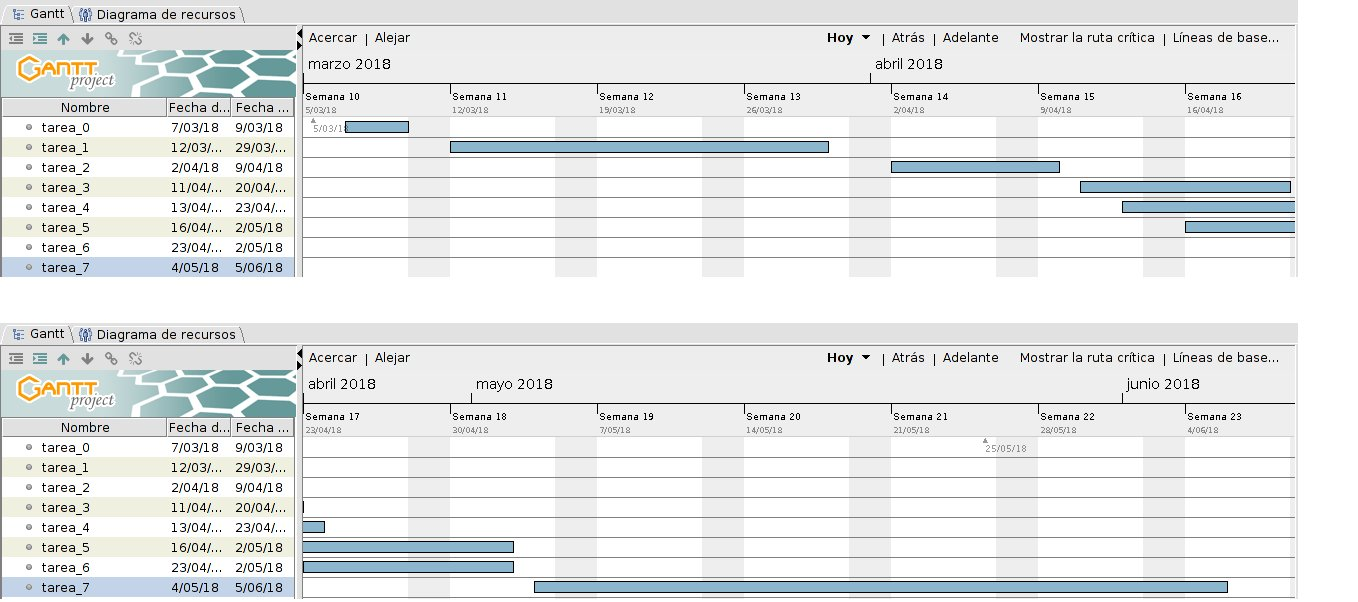
\includegraphics[width=1.5\textwidth, angle=90]{imagenes/gantt.jpg}
	\label{fig:gantt}
	\caption{Diagrama de Gantt.}
\end{figure}

\begin{table}[!h]
	\centering
	\begin{tabular}{|p{2cm} | p{5cm} | p{2cm} | p{2cm} | p{2cm} |}
		\hline
		\textbf{Tarea} & \textbf{Nombre} & \textbf{Fecha de inicio} & \textbf{Fecha de fin} & \textbf{Estimación} \\
		\hline
		tarea\_0 & Instalación y toma de conceptos de MoveIt! y ROS & 07/03/2018 & 10/03/2018 & 4 días\\
		\hline
		tarea\_1 & Adaptación de software \textit{pick and place} utilizando módulos de visión & 12/03/2018 & 30/03/2018 & 18 días \\
		\hline
		tarea\_2 & Estudio de visión por computador & 02/04/2018 & 10/04/2018 & 8 días \\
		\hline
		tarea\_3 & Estudio de algoritmo k-medias e implementación en C++ & 11/04/2018 & 21/04/2018 & 10 días \\
		\hline 
		tarea\_4 & Desarrollo de software de visión por computador & 13/04/2018 & 23/04/2018 & 10 días \\
		\hline
		tarea\_5 & Desarrollo de software de clasificación en entorno estático & 16/04/2018 & 03/04/2018 & 17 días \\
		\hline
		tarea\_6 & Desarrollo de software de clasificación en entorno dinámico & 23/04/2018 & 03/05/2018 & 11 días \\
		\hline
		tarea\_7 & Realización de pruebas y corrección de errores & 04/05/2018 & 06/06/2018 & 30 días \\
		\hline
		
	\end{tabular}
	\caption{Planificación de proyecto.}
	\label{cuad:plan}
\end{table}

\newpage
\subsection{Presupuesto}

\subsubsection{Recursos hardware y software}

\noindent Para hacer el presupuesto de este proyecto se ha utilizado la fórmula siguiente:
\begin{center}
	$ (D/V) * C $
\end{center}

\noindent Donde:
\begin{itemize}
	\item D es el número de meses que se ha utilizado el producto para el proyecto.
	\item V es la vida útil del producto en número de meses.
	\item C es el coste total del producto en euros. \\
\end{itemize}

\begin{table}[H]
	\centering
	\begin{tabular}{|p{2cm} | p{2cm} | p{2cm} | p{2cm} | p{2cm} |}
		\hline % para poner una linea horizontal
		\textbf{Artículo} & \textbf{Coste} (euros) & \textbf{Dedicación} (meses) & \textbf{Vida Útil} (meses) & \textbf{Coste Aplicable} (euros)\\ % el & se usa para separar columnas y el \\ para saltos de linea
		\hline	
		Baxter & 24078\euro & 4 & 120 & 802,6\euro \\
		\hline
		Ordenador de sobremesa & 1500\euro & 4 & 60 & 100\euro \\
		\hline
		Cinta transportadora & 350\euro & 2 & 120 & 5,83\euro \\
		\hline
		Total & \multicolumn{4}{r|}{868,43\euro} \\ 
		\hline
	\end{tabular}
	\caption{Tabla de costes.}
\end{table}

\subsubsection{Recursos humanos}
\noindent En este trabajo se han empleado aproximadamente 80 días, contando con que una jornada laboral común suelen ser 8 horas al día y con que además de este proyecto se ha trabajado en otras asignaturas, se considera que en media se han invertido 4 horas al día. \\

\noindent Suponiendo que un ingeniero informático recién graduado en España representa un coste de 2000 euros al mes, las 320 horas del proyecto estarían valoradas en 1731.2 euros en total. \\


\subsubsection{Coste total}
\begin{table}[H]
	\centering
	\begin{tabular}{|p{4cm} | p{4cm} |}
		\hline
		\multicolumn{2}{|c|}{\textbf{COSTE TOTAL}} \\
		\hline 
		Recursos HW y SW & 868\euro \\
		\hline
		Recursos humanos & 1731\euro \\
		\hline
		Coste total & 2599\euro \\
		\hline
	\end{tabular}
	\caption{Coste total del proyecto}
	\label{cuad:ct}
\end{table}

\noindent Por lo tanto, añadiendo un 20\% referido a gastos, el coste total del proyecto sería de: \\

PRECIO TOTAL: 3120\euro (IVA no incluido)\\

\subsection{Gestión de problemas}
\label{planif}
\noindent En este proyecto se han enfrentado muchos problemas de los que se hablará en este apartado. Se hacía imprescindible su resolución, ya que suponían un impacto grave en el funcionamiento del código.\\

\noindent \textbf{Problema 1. Incompatibilidades a la hora de utilizar las plataformas MoveIt!, Gazebo y ROS sobre Ubuntu 16.04 LTS en el portátil personal.} No se propuso ninguna solución, puesto que en el laboratorio había un servidor disponible con Ubuntu 14.04.5 LTS y ROS Indigo. \\

\noindent \textbf{Problema 2. Actualización en el servidor del laboratorio.} Debido a una actualización de Windows, la gráfica de este computador quedó inutilizable. Para resolver este problema, se formateó el servidor, instalando ROS Kinetic sobre Ubuntu 16.04 LTS y MoveIt! (esta vez no resultó necesario instalar el simulador Gazebo, ya que este servidor se encuentra en el mismo lugar que el robot Baxter). \\

\noindent \textbf{Problema 3. Planificación de MoveIt!.} A la hora de utilizar OMPL, el algoritmo de planificación de MoveIt!, el resultado obtenido no siempre es el esperado; en ocasiones, al intentar ejecutar movimientos simples, el algoritmo recalcula la posición de las articulaciones de Baxter de forma que esta sea la óptima, sin embargo, resulta en un movimiento del brazo robótico más espaciado que impide realizar la clasificación correctamente. Para solucionarlo se implementan como movimientos pequeñas variaciones con respecto a la posición que el brazo tenía anteriormente.\\

%\noindent A la hora de la separación, cuando el \textit{gripper} de Baxter ya se encontraba en el punto medio, surgía otro problema al rotar el \textit{gripper} hacia la posición horizontal, ya que este giraba en el mismo sentido en todas las ocasiones. Esto no siempre era un problema, ya que algunas ejecuciones dejaban el brazo en el mejor caso posible, pero resultaba muy ineficiente en los casos en los que no era así. \\
%\noindent Esto podía resolverse comprobando si la orientación superaba $\pi$/4, en ese caso cambiabamos el sentido de la orientación.\\

%\noindent Baxter muy lento

\noindent \textbf{Problema 4. Permisos de ejecución.} ROS suele expresar los errores como \textit{``Process is dead''}. Normalmente especifica anteriormente el porqué, pero en este caso no lo hacía. El problema era que el programa escrito en Python no tenía permisos de ejecución. \\


\noindent \textbf{Problema 5. Iluminación.} La iluminación es una característica clave en un programa que utiliza visión por computador, y son muchos los problemas que esta puede dar, un ejemplo son los focos, ya que aunque no los veamos, están parpadeando constantemente, esto influye al capturar las imágenes de los objetos. Existen focos de luz azul capaces de solucionar esto; en mi caso, utilicé la luz natural y alguna artificial de la sala, intentando crear sombras para que esta no incidiese directamente sobre los objetos.\\

\noindent \textbf{Problema 6. Entrada del algoritmo K-means.} El problema principal consistía en que el único tipo de dato que se le puede pasar a este algoritmo es \textit{Mat} de OpenCV. Puesto que se estaba trabajando con \textit{PoseArray} de ROS para obtener las coordenadas en la imagen, se intentó adaptar para pasárselo a K-means. Este consiste en un array de \textit{PoseStamped}, un tipo de dato que incluye unas coordenadas para especificar la posición del objeto y otras para la orientación. Puesto que el objetivo más básico del proyecto era realizar una segmentación por color y posición y al algoritmo no se le podían pasar valores RGB ya que la salida resultaría ser otro valor intermedio RGB y no una posición entre los dos clústers, se definió específicamente un valor para cada objeto que indicaba su color y se mandaba a través de la coordenada \textit{z}, ya que no es necesario especificarla porque los objetos siempre se mantienen en la misma \textit{z} (sobre la mesa o cinta transportadora). Así, la posición, orientación y color del objeto se incluyen en la matriz \textit{Mat} para obtener los dos clústers tras ejecutar K-means.\\